\documentclass[tikz,border=10pt]{standalone}
\usepackage{amsmath,amssymb}
\usepackage{tikz}
\usetikzlibrary{arrows,automata,backgrounds,calendar,chains,decorations,decorations.pathreplacing,decorations.text,fit,matrix,mindmap,patterns,petri,plotmarks,positioning,shadows,shapes,shapes.callouts,shapes.geometric,shapes.misc,spy,trees,calc,intersections,tikzmark,arrows.meta}
\usepackage{xcolor}
\usepackage{pgfplots}
\pgfplotsset{compat=1.16}

% Common math macros from the book
\def\x{\mathbf{x}}
\def\y{\mathbf{y}}
\def\z{\mathbf{z}}
\def\A{\mathbf{A}}
\def\b{\mathbf{b}}
\def\c{\mathbf{c}}
\def\w{\mathbf{w}}
\def\v{\mathbf{v}}
\def\u{\mathbf{u}}
\def\e{\mathbf{e}}
\def\zero{\mathbf{0}}
\def\R{\mathbb{R}}
\def\N{\mathbb{N}}
\def\Z{\mathbb{Z}}
\def\Q{\mathbb{Q}}
\def\st{\text{s.t.}}
\def\vect#1{\mathbf{#1}}
\def\xLP{x^{\mathrm{LP}}}
\def\zLP{z^{\mathrm{LP}}}
\def\xIP{x^{\mathrm{IP}}}

% Common node styles from the book
\tikzset{
    main/.style={circle, draw, fill=gray!20, minimum size=1cm, font=\normalsize},
    dot/.style={circle,fill=blue,minimum size=3pt,inner sep=0pt, outer sep=-1pt},
    vertex/.style={circle,fill=black!25,minimum size=20pt,inner sep=0pt},
    edge/.style={draw,-,thick},
    directed edge/.style={draw,->,>=latex,thick},
}

% Additional macros for 3D/coordinate systems
\newcommand{\xhat}{\hat{\x}}
\newcommand{\yhat}{\hat{\y}}
\newcommand{\zhat}{\hat{\z}}
\newcommand{\ihat}{\hat{\imath}}
\newcommand{\jhat}{\hat{\jmath}}
\newcommand{\khat}{\hat{k}}

\begin{document}
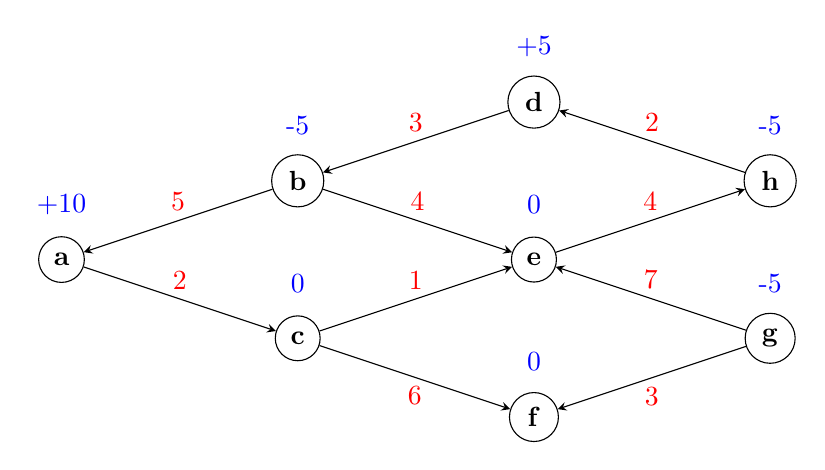
\begin{tikzpicture}[>=stealth, node distance=3cm]

    % Nodes (circled)
    \node[draw, circle] (a) at (0,6) {\textbf{a}};
    \node[draw, circle] (b) at (3,7) {\textbf{b}};
    \node[draw, circle] (c) at (3,5) {\textbf{c}};
    \node[draw, circle] (d) at (6,8) {\textbf{d}};
    \node[draw, circle] (e) at (6,6) {\textbf{e}};
    \node[draw, circle] (f) at (6,4) {\textbf{f}};
    \node[draw, circle] (g) at (9,5) {\textbf{g}};
    \node[draw, circle] (h) at (9,7) {\textbf{h}};

    % Net flow annotations (above nodes, in blue)
    \node[blue] at (0,6.7) {+10};
    \node[blue] at (3,7.7) {-5};
    \node[blue] at (3,5.7) {0};
    \node[blue] at (6,8.7) {+5};
    \node[blue] at (6,6.7) {0};
    \node[blue] at (6,4.7) {0};
    \node[blue] at (9,5.7) {-5};
    \node[blue] at (9,7.7) {-5};

    % Edges with costs (in red)
    \draw[->] (b) -- (a) node[midway, above,  red] {5};
    \draw[->] (a) -- (c) node[midway, above,  red] {2};
    \draw[->] (d) -- (b) node[midway, above,  red] {3};
    \draw[->] (b) -- (e) node[midway, above,  red] {4};
    \draw[->] (c) -- (e) node[midway, above,  red] {1};
    \draw[->] (c) -- (f) node[midway, below,  red] {6};
    \draw[->] (h) -- (d) node[midway, above,  red] {2};
    \draw[->] (g) -- (e) node[midway, above,  red] {7};
    \draw[->] (e) -- (h) node[midway, above,  red] {4};
    \draw[->] (g) -- (f) node[midway, below,  red] {3};
    
\end{tikzpicture}
\end{document}
